\chapter{Funkcionalnosti}
Kako oba alata imaju pregršt funkcionalnosti navesti ću njihove najzanimljivije i najbolje implementirane funkcionalnosti 
koje će kasnije biti uspoređene.
\section{OWASP ZAP}
OWASP ZAP (još znan i kao Zed Attack Proxy) je program otvorenog koda namijenjen
za skeniranje web aplikacija tj.\ stranica. Produkt je organizacije \textit{Open Web Application 
Security Project} (OWASP) te održavan kako od njih tako i od nemale skupine programera 
i sigurnosnih stručnjaka iz cijelog svijeta. Alat pruža široki skup mogućnosti 
za detekciju i testiranje ranjivosti u web aplikacijama. Izgled ZAPa pri njegovom pokretanju vidljiv je na slici \ref{slk:owasp_start}.
\begin{figure}[H]
    \centering
    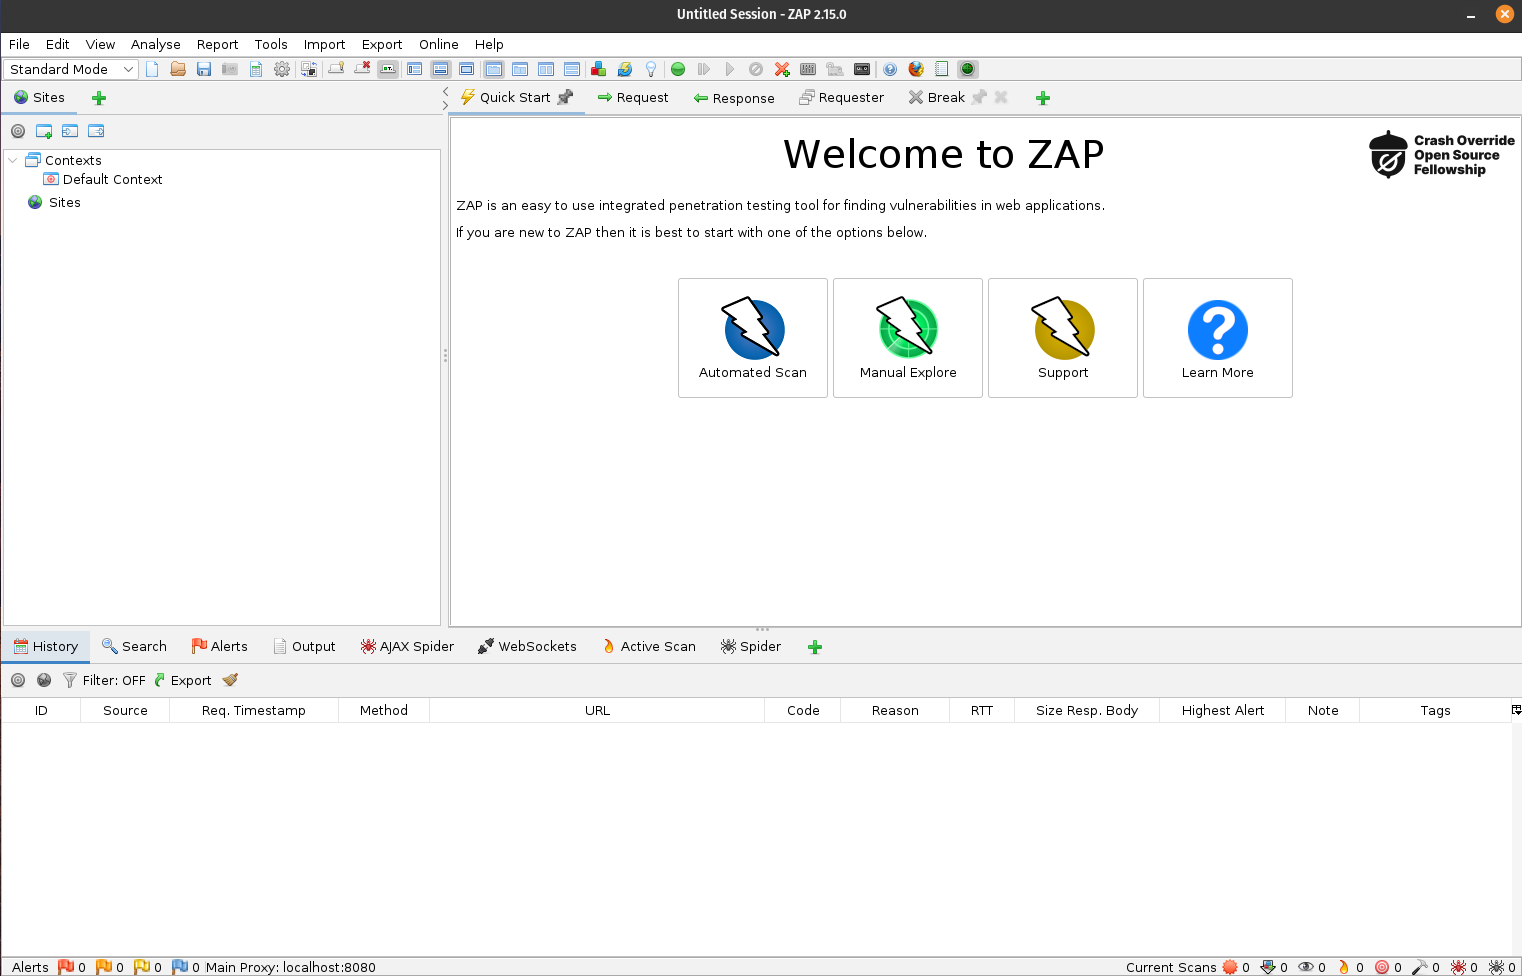
\includegraphics[width=0.8\textwidth]{slike/zap_start.png}
    \caption{Izgled OWASP ZAP-a pri pokretanju}
    \label{slk:owasp_start}
  \end{figure}

\subsection{Presretački \textit{proxy}}
\textit{Intercepting Proxy}, poznat i kao \textit{"Break"} u \textit{OWASP ZAP}-u, ključna je funkcionalnost koja omogućava 
korisnicima da presreću i pregledavaju \textit{HTTP/HTTPS} zahtjeve i odgovore između preglednika i web aplikacije. Ovo omogućuje 
korisnicima da detaljno pregledaju i modificiraju podatke prije nego što su oni poslani na server ili primljeni u pregledniku. 
Presretanje prometa korisno je za ručno testiranje sigurnosti jer omogućuje detaljnu analizu 
\textit{HTTP} zahtjeva i odgovora, uključujući zaglavlja, kolačiće, tijela zahtjeva i odgovore. 
Prije nego što se zahtjev pošalje ili odgovor primi, korisnici mogu ručno promijeniti podatke 
kako bi testirali različite scenarije.

Integrirani \textit{Heads-Up Display (HUD)} omogućava vizualno praćenje i kontrolu presretanja 
prometa direktno iz preglednika. Korisnici mogu simulirati razne vrste napada presretanjem i 
modificiranjem prometa, kao što su \textit{SQL} injekcije, \textit{XSS} napadi, \textit{CSRF}, i 
druge.\cite{ZAP_docs,zap_feat}


\subsection{Aktivno i pasivno skeniranje}% (engl. \textit{Active and Passive scan})}
Aktivno skeniranje (\textit{Active scan}) je ispitivanje ranjivosti pri kojem ZAP aktivno interaktira s aplikacijom ne bi li 
otkrila sve potencijalne sigurnosne prijetnje. Skeniranje uključuje slanje zahtjeva sistemu koji se testira (eng. \textit{system under test}, 
nadalje SUT) te analiziranje odgovora ne bi li dobili uvid u ranjivosti aplikacije.

Pasivno skeniranje (\textit{Passive scan}) je tip skeniranja gdje ZAP ne interaktira direktno s ijednim dijelom sustava na ijedan način.
Kako bi se pasivno prikupljale informacije, alat nadgleda mrežni promet za potencijalne ranjivosti. U pozadini alat i dalje nadgleda zahtjeve 
i odgovore no ne zamarajući korisnika s njima sve dok ne otkrije problem, onda podigne \textit{alert}.

Dobra stvar kod skeniranja u ZAP-u je mogućnost kontrole politike skeniranja. Ona nam omogućava da alatu pomognemo da bolje, lakše i brže pronađe ranjivosti koristeći 
znanje koje mi trenutno imamo, mogućnosti hardwera s kojim testiramo te vrste skenera koje imamo na raspolaganju. Te se politike mogu spremati te kasnije koristiti kao 
predložak u budućem testiranju.\cite{ZAP_docs,zap_feat}

\subsection{Skeniranje portova} % (engl. \textit{Port Scan})}
Funkcionalnost skeniranja portova u \textit{OWASP ZAP}-u obavlja skeniranje ranjivih portova nad \textit{SUT}-om kako bi utvrdio 
ranjive portove. U svojoj suštini radi isto što i određeni testovi za \textit{Nmap}\cite{nmap}, pronalazeći otvorene i zatvorene 
portove. Također, kao i \textit{Nmap}, može pronaći koji je trenutni servis na nekom od portova.

Služi kako bi se dobile dodatne informacije o potencijalnim vektorima napada. Pored toga, \textit{OWASP ZAP} može integrirati 
rezultate skeniranja portova sa svojim ostalim alatima za sigurnosno testiranje, omogućujući sveobuhvatnu analizu sigurnosti.

Za korištenje ove funkcionalnosti, potrebno je omogućiti \textit{Port Scanner} dodatak u \textit{OWASP ZAP}-u. 
Nakon omogućavanja, korisnici mogu konfigurirati skeniranje da cilja specifične portove ili opsege portova, prilagoditi vrijeme 
čekanja na odgovore, i odabrati protokole nad kojima će se testirati.\cite{zap_feat}

\subsection{Aplikacijsko programsko sučelje}
\textit{API} omogućava korisnicima programski pristup direktno kodu tj. njegovoj funkcionalnosti. API omogućava automatizaciju određenih aspekata web testiranja te 
integraciju s ostalim alatima.

Proširivost \textit{ZAP}-a je upravo ono što ga čini toliko moćnim naspram drugih alata. \textit{ZAP API} podržava više jezika, uključujući \textit{Python}, \textit{Javu}, \textit{JavaScript}, \textit{Ruby}, i druge, što omogućava široku primjenu u različitim okruženjima. 
Kroz \textit{API}, korisnici mogu pokretati skeniranja, pristupati rezultatima, mijenjati postavke i čak kreirati prilagođene napade.
\textit{ZAP API} se može koristiti za kontinuiranu integraciju (\textit{CI}) i kontinuiranu isporuku (\textit{CD}), omogućavajući sigurnosno testiranje kao dio razvojnih procesa. 
Integracija s alatima kao što su \textit{Jenkins} i \textit{GitLab CI} omogućava automatsko pokretanje sigurnosnih skeniranja prilikom svakog \textit{build}-a, čime se osigurava otkrivanje potencijalnih ranjivosti ranije u procesu.
Također, \textit{ZAP API} omogućava jednostavno skaliranje testiranja. Korisnici mogu pokretati paralelna skeniranja na različitim ciljevima, što ubrzava proces testiranja velikih aplikacija. 
\textit{API} podržava sve glavne funkcionalnosti \textit{ZAP}-a, uključujući \textit{Spider}, \textit{Active Scan}, \textit{Passive Scan}, \textit{Forced Browse}, i druge, čime se omogućava sveobuhvatno testiranje kroz automatizirane skripte.

Dokumentacija za \textit{ZAP API} je detaljna i pruža primjere za korištenje u različitim programskim jezicima, što olakšava integraciju i korištenje čak i za one koji nisu stručnjaci za sigurnost.\cite{zap_feat}

\subsection{\textit{Fuzzer}}
\textit{OWASP ZAP fuzzer} stvara jedinstvene zahtjeve (engl. \textit{payloads}) koje potom šalje na \textit{SUT} koristeći već postojeće zahtjeve kao početnu odnosno 
referentnu točku. Fuzzer ima četiri načina rada: \textit{safe}, \textit{protected}, \textit{standard}, i \textit{ATTACK}. Svaki od navedenih načina pruža drukčije 
funkcionalnosti te načine rada.
\textit{OWASP ZAP fuzzer} također omogućava korisnicima da prilagode i kreiraju vlastite zahtjeve za specifične testove. Korisnici mogu definirati različite uzorke, 
vrijednosti i sekvence koje će se koristiti u \textit{fuzzing} procesu. \textit{Fuzzer} je integriran sa ostalim alatima u \textit{ZAP}-u, omogućujući kombiniranje rezultata i sveobuhvatnu 
analizu.
\textit{ZAP fuzzer} pruža detaljne izvještaje o rezultatima fuzzing testa, uključujući sve pronađene ranjivosti, odgovore servera, i potencijalne sigurnosne probleme. 
Ova funkcionalnost je ključna za dubinsko testiranje i identifikaciju skrivenih ranjivosti u web aplikacijama.\cite{ZAP_docs}

\subsection{Trgovina ekstenzija (engl. \textit{Marketplace})}
%Iako nije vezan direktno za web sigurnost \textit{Matketplace} je jako dio bitan ZAP-a. Omogućava korisnicima da prošire funkcionalnosti koje ZAP pruža sa ekstenzijama pisane od strane programera diljem svijeta pritom iskorištavajući sustav ocjenjivanja kao i metriku preuzimanja kako bi osigurao da se najviše predlažu najbolje ekstenzija.
\textit{Marketplace}, iako nije direktno povezan s web sigurnošću, predstavlja vrlo važan dio ZAP-a. Omogućuje korisnicima proširenje funkcionalnosti ZAP-a 
putem ekstenzija koje su razvili programeri iz cijelog svijeta. Sustav ocjenjivanja i metrike preuzimanja osiguravaju preporuku najkvalitetnijih ekstenzija.

Upravo zbog ove funkcionalnosti je ZAP uspio dobiti reputaciju kakvu trenutno ima. Zbog jednostavnosti modificiranja te principa otvorenog koda ambiciozna zajednica ljudi se brzo okupila kako bi pretvorili ovaj besplatan alat u sveobuhvatnog suradnika pri testiranju web aplikacija.\cite{zap_feat}

\newpage
\section{Burp Suite}
Uz ZAP postoji Burp Suite, stariji i komercijalni alat namijenjen za sigurnosno testiranje 
web aplikacija. Burp suite je razvila kompanija PortSwigger koja se također brine za njegovo 
održavanje. Burp suite omogućuje pristup velikom rasponu alata, od skenera za traženje ranjivosti 
pa sve do naprednih alata za \textit{fuzzing} i analizu web aplikacija. Početni prozor programa možemo vidjeti na slici \ref{slk:burp_start}.
Ovdje su pri vrhu vidljive kartice za određene module, lijevo se nalaze takozvani \textit{live taskovi}, u sredini su pronađene ranjivosti, a desno konfiguracija \textit{live taskova}.
\begin{figure}[H]
    \centering
    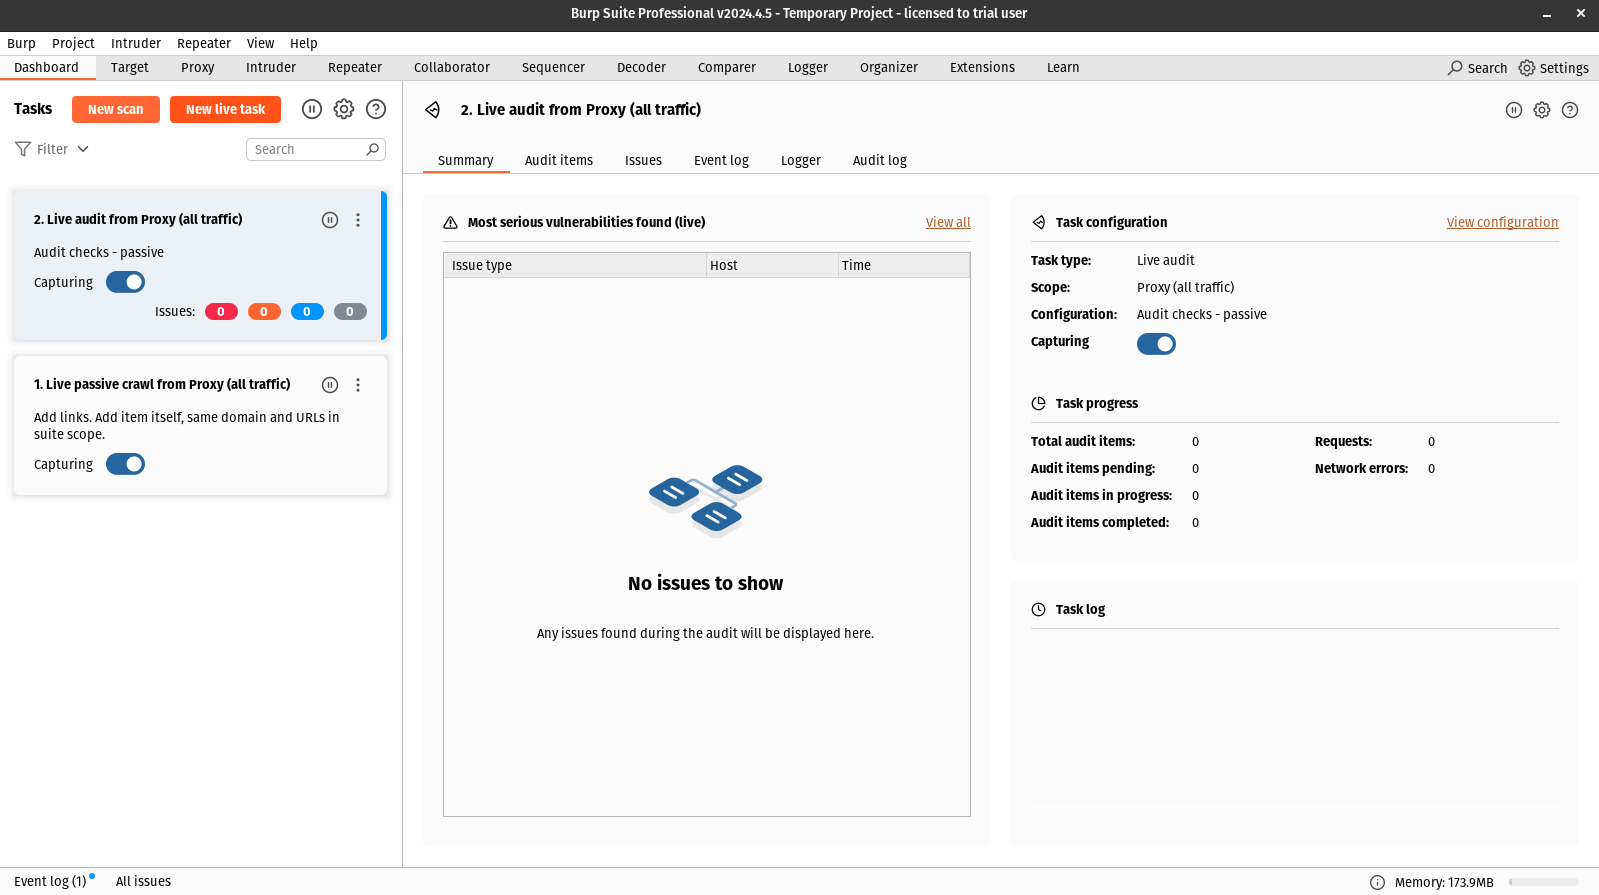
\includegraphics[width=1\textwidth]{slike/burp_start.png}
    \caption{Izgled Burp suita pri pokretanju}
    \label{slk:burp_start}
\end{figure}
\subsection{\textit{Proxy}}
Burp \textit{Proxy} je jedan od glavnih modula Burp Suitea. On omogućava presretanje, pregled i promjenu HTTP i HTTPS zahtjeva između preglednika i web aplikacije. 
Koristeći Proxy, sigurnosni stručnjaci mogu analizirati zahtjeve i odgovore, tražiti ranjivosti i manipulirati podacima kako bi testirali sigurnost web aplikacije.\cite{burp_feat}

\subsection{\textit{Intruder}}
Burp \textit{Intruder} je modul za automatizirane napade. Može se koristiti za \textit{brute force} napade, testiranje valjanosti unosa, traženje skrivenih direktorija ili datoteka, 
te druge vrste napada. Korisnik može konfigurirati različite parametre i payload-ove koji će se automatski slati, a Intruder će analizirati odgovore kako bi identificirao 
potencijalne ranjivosti.\cite{burp_feat}

\subsection{\textit{Repeater}}
\textit{Repeater} omogućava korisnicima da ponavljaju HTTP/HTTPS zahtjeve ručno. Ovo je korisno za detaljno testiranje specifičnih zahtjeva i odgovora. Korisnik može modificirati i 
ponovo poslati zahtjeve, te analizirati odgovore kako bi identificirao ranjivosti i prijetnje.\cite{burp_feat}

\subsection{\textit{Collaborator}}
\textit{Collaborator} je modul za otkrivanje server-side ranjivosti koje zahtijevaju interakciju s vanjskim sustavima/stranicama. Primjeri ovih ranjivosti uključuju 
SSRF (engl. \textit{Server-Side Request Forgery}) i različite vrste injekcija koje rezultiraju vanjskim interakcijama. Omogućava postavljanje posebnog servera koji prati 
ove interakcije i pomaže u identifikaciji ranjivosti.\cite{burp_feat}

\subsection{\textit{Comparer}}
\textit{Comparer} omogućava uspoređivanje dva skupa podataka. Ovo može biti korisno za analizu promjena između dva odgovora ili zahtjeva, kako bi se identificirale suptilne razlike koje 
mogu ukazivati na ranjivosti kao što su neodgovorna obrada zahtjeva pri kojoj mogu iscuriti informacije iz takozvanih 'sporednih kanala'. \cite{burp_feat}

\subsection{\textit{Extensions}}
\textit{Extensions} modul omogućava proširivanje funkcionalnosti Burp Suitea putem dodataka (ekstenzija). Korisnici mogu instalirati ekstenzije iz BApp Storea ili kreirati 
vlastite koristeći Burp Extender API. Ovo omogućava prilagođavanje alata specifičnim potrebama i dodavanje novih funkcija koje nisu dostupne u osnovnoj verziji.\cite{burp_feat}


\newpage
\section{Usporedba alata \textit{a priori}}
U svojoj suštini ZAP i Burp suite Professional imaju iste funkcionalnosti. Kroz godine su OWASP i nezavisni programeri polako gradili alat koji sada već može parirati profesionalnom
plaćenom alatu.
Kao što se iz tablice \ref{tbl:usporedba} zaključiti ZAP po svemu parira Burp suite-u, no i dalje oba alata imaju prednosti i mana. Jedna od većih mana Burp Professional Suita je njegova cijena gdje će nas samo jedna godina licence koštati 450 eura.
Manjkavost ZAP-a je \textit{Fuzzer}. U trenutku izrade rada funkcionalnost tog modula nije u potpunosti realizirana kao kod Burp-a što će kasnije biti pokazano.
Funkcionalnosti koje ZAP ima a Burp suite nema su mogućnost automatizacije i HUD (engl. \textit{Heads Up Display}). Automatizaciju ZAP sam prije spomenuo a HUD ću koristiti i objasniti prilikom testiranja.
Što se tiče korisničkog sučelja oba alata pružaju lijepo i moderno sučelja, gdje Burp ima malu prednost zbog jasnoće i intuitivnosti kartica i modula.
\begin{table}[H]
  \centering
  \caption{Burp suite modul i odgovarajuća alternativa realizirana u ZAP-u\cite{burp_to_zap}}
  \begin{tabular}{|c|c|}
      \hline
      \textbf{Burp Suite Professional značajka} & \textbf{ZAP alternativa} \\
      \hline
      Collaborator & OAST Support Add-on \\
      Comparer & Diff \\
      Decoder & Encoder \\
      DOM Invader & Eval Villian ekstenzija \\
      Extender & Marketplace, Scripts \\
      Intercept & Breakpoints \\
      Intruder & Fuzzer\textbf{*} \\
      Live scan & ATTACK Mode \\
      Project Files & Session Files \\
      Proxy & Proxy \\
      Repeater & Manual Request Editor, Requester ekstenzija \\
      Scanner & Active Scanner \\
      Sequencer & Token Generation and Analysis \\
      Target & Contexts \\
      \hline
  \end{tabular}
\label{tbl:usporedba}
\end{table}